\documentclass{article}
\usepackage[utf8]{inputenc}
\usepackage{ebproof}
\usepackage{amsmath}
\usepackage{ebproof}
\usepackage{virginialake}
\usepackage{cmll}
\usepackage{tikz}

\parindent=0pt
\parskip=0.6em

\usepackage{amsthm}\theoremstyle{plain}
\newtheorem{thm}{Theorem}[section]

\theoremstyle{definition}
\newtheorem{definition}[thm]{Definition}
\newtheorem{lemma}[thm]{Lemma}
\newtheorem{notation}[thm]{Notation}
\newtheorem{proposition}[thm]{Proposition}
\newtheorem{theorem_}[thm]{Theorem}
\newtheorem{example}[thm]{Example}
\newtheorem{remark}[thm]{Remark}

\title{On first-order combinatorial proofs}
\author{Jui-Hsuan Wu, Lutz Strassburger}

\begin{document}

\maketitle

\section{From first-order logic to combinatorial proofs}

\subsection{{\bf LK}}
We start with Gentzen's sequent calculus system {\bf LK}.

\begin{center}

\mbox{
\begin{prooftree}
  \infer0[$ax$]{\vdash A, \neg A}
\end{prooftree}
\hspace{2cm}

\begin{prooftree}
  \hypo{\vdash \Gamma, A}
  \hypo{\vdash \Delta, \neg A}
  \infer2[$cut$]{\vdash \Gamma, \Delta}
\end{prooftree}}

\mbox{
\begin{prooftree}
  \hypo{\vdash \Gamma, A}
  \hypo{\vdash \Delta, B}
  \infer2[$\wedge$]{\vdash \Gamma, \Delta, A \wedge B}
\end{prooftree}
\hspace{1.5cm}

\begin{prooftree}
  \hypo{\vdash \Gamma, A, B}
  \infer1[$\vee$]{\vdash \Gamma, A \vee B}
\end{prooftree}}

\mbox{
\begin{prooftree}
  \hypo{\vdash \Gamma, A, A}
  \infer1[$ctr$]{\vdash \Gamma, A}
\end{prooftree}
	\hspace{2cm}

\begin{prooftree}
  \hypo{\vdash \Gamma}
  \infer1[$wk$]{\vdash \Gamma, A}
\end{prooftree}}

\mbox{
\begin{prooftree}
\infer0[$\ttt$]{\vdash \ttt}
\end{prooftree}
\hspace{2cm}

\begin{prooftree}
  \hypo{\vdash \Gamma}
	\infer1[$\fff$]{\vdash \Gamma, \fff}
\end{prooftree}}

\mbox{
\begin{prooftree}
  \hypo{\vdash \Gamma, A}
  \infer1[$\forall$]{\vdash \Gamma, \forall x A}
\end{prooftree}
($x \notin fv(\Gamma)$)
\hspace{2cm}

\begin{prooftree}
  \hypo{\vdash \Gamma, A[t/x]}
  \infer1[$\exists$]{\vdash \Gamma, \exists x A}
\end{prooftree}}

\end{center}

We also consider the mix rule here:

\begin{center}
\begin{prooftree}
\hypo{\vdash \Gamma}
\hypo{\vdash \Delta}
\infer2[$mix$]{\vdash \Gamma, \Delta}
\end{prooftree}
\end{center}

Note that the mix rule is derivable via weakening in {\bf LK}.

Consider the following deep rules:
\begin{center}
\mbox{
\begin{prooftree}
  \hypo{\vdash S\{A \vee A\}}
  \infer1[$\cD$]{\vdash S\{A\}}
\end{prooftree}
\hspace{2cm}

\begin{prooftree}
  \hypo{\vdash S\{\fff \}}
  \infer1[$\wD$]{\vdash S\{A\}}
\end{prooftree}
}
\end{center}


Note that the $ctr$ (resp. $wk$) rule in {\bf LK} is derivable in $\{\cD, \vee\}$
(resp. $\{\wD, \fff\}$) and that $\cD$ and $\wD$ rules
permute downwards with the non-structural rules of {\bf LK}. 

\begin{center}
\mbox{

\begin{prooftree}
  \hypo{\vdash \Gamma, A, A}
  \infer1[$ctr$]{\vdash \Gamma, A}
\end{prooftree}

$\ \leadsto \ $

\begin{prooftree}
  \hypo{\vdash \Gamma, A, A}
  \infer1[$\vee$]{\vdash \Gamma, A \vee A}
  \infer1[$\cD$]{\vdash \Gamma, A}
\end{prooftree}}
\vspace{0.2cm}

\mbox{
\begin{prooftree}
  \hypo{\vdash \Gamma}
  \infer1[$wk$]{\vdash \Gamma, A}
\end{prooftree}

$\ \leadsto \ $

\begin{prooftree}
  \hypo{\vdash \Gamma}
  \infer1[$\fff$]{\vdash \Gamma, \fff}
  \infer1[$\wD$]{\vdash \Gamma, A}
\end{prooftree}}

\end{center}

We also give an example to show how rule permutation works:

\begin{center}

\mbox{
\begin{prooftree}
\hypo{\Gamma,A \vee A}
\infer1[$\cD$]{\Gamma,A} 
\hypo{\Delta,B}
\infer2[$\wedge$]{\Gamma, \Delta, A \wedge B} 
\end{prooftree}

$\ \leadsto \ $

\begin{prooftree}
\hypo{\Gamma,A \vee A}
\hypo{\Delta,B}
\infer2[$\wedge$]{\Gamma, \Delta, (A \vee A) \wedge B} 
\infer1[$\cD$]{\Gamma, \Delta, A \wedge B} 
\end{prooftree}}

\end{center}

We want to establish the following theorem:

\begin{theorem_}
\label{thm1}
Let $\Gamma$ be a sequent. Then there is a proof of $\Pi$ in {\bf LK} + $mix$ iff there is a proof of some sequent $\Delta$ in {\bf MLL1} + $mix$ and a derivation from $\Delta$ to $\Gamma$ consisting of the $\cD$ and $\wD$ rules only. 
\end{theorem_}

\begin{proof}
($\Rightarrow$) This direction comes from the above observation: it suffices to permute downwards all the instances of the $\cD$ and $\wD$ rules.

($\Leftarrow$)
We regard the proof in {\bf MLL1} + $mix$ as a proof in {\bf LK} + $mix$.
Then we put the derivation consisting of only $\cD$ and $\wD$ under the proof in {\bf LK} + $mix$. Now we try to permute all the instances $\cD$ and $\wD$ upwards with the rules of LK and $mix$. 
For the $\cD$ part, the only non-trivial case is the permutation with the $\vee$ rule where the formula generated is $A \vee A$.

\begin{center}
\mbox{
\begin{prooftree}
\hypo{\vdash \Gamma, A, A}
\infer1[$\vee$]{\vdash \Gamma, A \vee A}
\infer1[$\cD$]{\vdash \Gamma, A}
\end{prooftree}

$\ \leadsto \ $

\begin{prooftree}
\hypo{\vdash \Gamma, A, A}
\infer1[$ctr$]{\vdash \Gamma, A}
\end{prooftree}

} 
\end{center}

In this case, the permutation of this instance of $\cD$ stops and we continue with the remaining instances.

For the $\wD$ part, the only non-trivial case is the permutation with the $\fff$ rule (or the instance of $wk$ where $\fff$ is introduced):

\begin{center}
\mbox{
\begin{prooftree}
\hypo{\vdash \Gamma}
\infer1[$\fff$]{\vdash \Gamma, f}
\infer1[$\wD$]{\vdash \Gamma, A}
\end{prooftree}

$\ \leadsto \ $

\begin{prooftree}
\hypo{\vdash \Gamma}
\infer1[$wk$]{\vdash \Gamma, A}
\end{prooftree}

} 
\end{center}

In this case, the permutation of this instance of $\wD$ stops and we continue with the remaining instances.

\end{proof}

\iffalse

Now consider a proof $\Pi$ of some sequent $\Gamma$ in {\bf LK}:
The observation above gives the possibility of
transforming the proof into a proof in {\bf MLL} followed by a derivation consisting
of the $\cD$ and $\wD$ rules only.

Conversely, consider a proof $\Pi$ of some sequent $\Gamma$ consisting of a
proof $\Pi'$ in {\bf LK} followed by a derivation $\Pi''$ consisting
the $\cD$ and $\wD$ rules only. 
We can assume that the proof $\Pi'$ is cut-free and contains only atomic
axioms.
Now consider some instance of $\cD$ in the derivation $\Pi''$:
\begin{prooftree}
  \hypo{S\{A \vee A\}} 
  \infer1[$\cD$]{S\{A\}}
\end{prooftree}

If the subformula $A \vee A$ is erased at some point by the $\wD$ rule: 

\begin{center}
\begin{prooftree}
  \hypo{\vdash T\{\fff\}}
  \infer1[$\wD$]{\vdash T\{B\}}
  \ellipsis{$\mathcal{D}$}{\vdash S\{A \vee A\}}
  \infer1[$\cD$]{\vdash S\{A\}}
\end{prooftree}
\end{center}

where $A \vee A$ is a subformula of $B$, then we can erase the instance of $\cD$
rule considered
and obtain the derivation:

\begin{center}
\begin{prooftree}
  \hypo{\vdash T\{\fff\}}
  \infer1[$\wD$]{\vdash T\{B[A \vee A \leftarrow A]\}}
  \ellipsis{$\mathcal{D}[A \vee A \leftarrow A]$}{\vdash S\{A\}}
\end{prooftree}
\end{center}

where $B[A \vee A \leftarrow A]$ (resp. $\mathcal{D}[A \vee A \leftarrow A]$) is the
formula (resp. derivation) obtained from $B$ (resp. $\mathcal{D}$) by replacing every
occurrence of $A \vee A$ with $A$.

Now suppose that the subformula $A \vee A$ is not erased in the derivation
$\Pi''$.

Since there is the contraction rule $ctr$, the subformula $A \vee A$ might be duplicated in the proof $\Pi'$. We now consider a branch of the proof $\Pi'$ 

Since $\Pi'$ is cut-free, it enjoys the subformula property and since all axioms
are atomic, the "subformula" $A \vee A$ should be decomposed at some point in the
proof and thus the proof $\Pi$ should be of the following form:

\begin{center}
\begin{prooftree}
  \hypo{\cdots}
  \hypo{\vdash \Gamma, A, A}
  \infer1[$\vee$]{\vdash \Gamma, A \vee A}
  \ellipsis{$\mathcal{D}$}{}
  \infer2[]{\vdash T\{A \vee A\}}
  \ellipsis{$\mathcal{D}_1$}{\vdash S\{A \vee A\}}
  \infer1[$\cD$]{\vdash S\{A\}}
  \ellipsis{$\mathcal{D}_2$}{\vdash \Gamma}
\end{prooftree}
\end{center}

where $\Pi'$ =
\begin{prooftree}
  \hypo{\vdash T\{A \vee A\}}
  \ellipsis{}{\vdash \Gamma}
\end{prooftree}

We can thus to apply the $ctr$ rule first and to replace each occurrence of $A
\vee A$ in the derivation (branch) $\mathcal{D}$:

\begin{center}
\begin{prooftree}
  \hypo{\cdots}
  \hypo{\vdash \Gamma, A, A}
  \infer1[$ctr$]{\vdash \Gamma, A}
  \ellipsis{$\mathcal{D}[A \vee A \leftarrow A]$}{}
  \infer2[]{\vdash T\{A \vee A\}}
  \ellipsis{$\mathcal{D}_1$}{\vdash S\{A \vee A\}}
  \infer1[$\cD$]{\vdash S\{A\}}
  \ellipsis{$\mathcal{D}_2$}{\vdash \Gamma}
\end{prooftree}
\end{center}

By applying the same process to all the branches of occurrences of $A \vee A$,
we obtain a proof of $\Gamma$ without the instance
\begin{prooftree}
  \hypo{S\{A \vee A\}}
  \infer1[$\cD$]{S\{A\}}
\end{prooftree}
of the $\cD$ rule. The derivation $\Pi'$ can be replaced by the following:
\begin{center}
\begin{prooftree}
  \hypo{\vdash T\{A\}}
  \ellipsis{$\mathcal{D}_1[A \vee A \leftarrow A]$}{\vdash S\{A\}}
  \ellipsis{$\mathcal{D}_2[A \vee A \leftarrow A]$}{\vdash \Gamma}
\end{prooftree}
\end{center}

We can thus eliminate all the instances of the $\cD$ rule in the proof. Suppose
now that the derivation $\Pi''$ consists of the $\wD$ rule only.

[PROOF TO DO]

\fi

D. Hughes proves the soundness and completeness of
unification nets with respect to {\bf MLL1} + $mix$. In the following, we establish the
equivalence between unification nets and fonets.

\subsection{Equivalence between unification nets and fonets}
In the following, we usually confound a vertex with its label. 

We also confound $\parr$ with $\vee$ and $\otimes$ with $\wedge$ as unification
nets and first-order nets (fonets) are defined in different contexts.

\begin{definition} A \textit{switching path} of a unification structure $U(\lambda)$ is a path in a switching graph of $U(\lambda)$.
\end{definition}

\begin{definition} A \textit{switching path} of a  formula tree $F(\phi)$ is a path in $F(\phi)$ that does not go through both incoming edges of a $\parr$.
\end{definition}

\begin{proposition}
\label{prop1}
In a formula tree, the root is connected to every vertex by a switching path.
\end{proposition}

Now we give the key proposition relating a fograph to its corresponding formula
tree.

\begin{proposition}
\label{prop2}
Let $u$ and $v$ be two distinct vertices of a fograph $G(\phi)$, then we have the equivalence
between:
\begin{itemize}
  \item $u$ and $v$ are adjacent in $G(\phi)$
  \item $u$ and $v$ are connected by a switching path of $F(\phi)$, and if one of them is a universal quantifier, then the other is
	not a descendant of the former.
  \end{itemize}
\begin{proof}
By induction on $\phi$.
\begin{itemize}
  \item If $\phi$ is an atom, trivial.
  \item If $\phi = \phi_1 \wedge \phi_2$, then we distinguish two cases:
    \begin{itemize}
      \item $u$ and $v$ are both in $\phi_1$ (resp. $\phi_2$): trivial by
	      the induction hypothesis.
      \item one of them is in $\phi_1$ and the other is in $\phi_2$: they are
	      adjacent in $G(\phi)$ by definition. By Proposition \ref{prop1},
		    the one in $\phi_1$ (resp. $\phi_2$) is connected to the
		    vertex representing $\phi_1$ (resp. $\phi_2$) by a switching
		    path. Together with the two edges incident to $\phi_1 \wedge
		    \phi_2$, we obtain a switching path connecting $u$ and $v$.
    \end{itemize}
  \item If $\phi = \phi_1 \vee \phi_2$, then we distinguish two cases:
    \begin{itemize}
      \item $u$ and $v$ are both in $\phi_1$ (resp. $\phi_2$): trivial by
	      the induction hypothesis.
      \item one of them is in $\phi_1$ and the other is in $\phi_2$: they are not
	      adjacent in $G(\phi)$ by definition. It is clear that they
		    are not connected by a switching path.
    \end{itemize}
  \item If $\phi = \exists x \ \phi'$, then we distinguish two cases:
    \begin{itemize}
      \item $u$ and $v$ are both in $\phi'$: trivial by the induction
	      hypothesis.
      \item one of them is $\exists x$ and the other is in $\phi'$: trivial
	      by Proposition \ref{prop1}

    \end{itemize}
  \item If $\phi = \forall x \ \phi'$, then we distinguish two cases:
    \begin{itemize}
      \item $u$ and $v$ are both in $\phi'$: trivial by the induction
	      hypothesis.
      \item one of them is $\forall x$ and the other is in $\phi'$:
	they are not adjacent in $G(\phi)$ by definition and it is clear that
		    the former is a descendant of $\forall x$.
    \end{itemize}
\end{itemize}
\end{proof}
\end{proposition}

\begin{proposition}
If there exists an induced bimatching of the linked fograph $G = G(\phi)$, then there exists a switching graph of the corresponding unification net which contains a cycle.
\begin{proof}
  Suppose that there exists a set $W$ inducing a bimatching in $G$.
  Then $(W, E_G)$ and $(W, L_G)$ are matchings.\\
  Let $E_W$ (resp. $L_W$) be the restriction of $E_G$ (resp. $L_G$) to $W$. \\
  If $E_W \cap L_W \neq \emptyset$, then there exist $u$ and $v$ such that $uv
  \in E_G$ and $uv \in L_G$. By Proposition \ref{prop2}, there exists a
  switching path of the formula tree of $\phi$. Together with the leap
  $uv$, this path induces a cycle in a switching graph of the
  corresponding unification structure. \\
  We can now suppose that $E_W$ and $L_W$ are disjoint. It is not difficult to
  see the existence of an alternating and elementary cycle  in the bicoloured graph $(W, E_W \uplus L_W)$, i.e. a cycle of which the edges are alternately in $E_W$ and $L_W$ and containing no two equal vertices.
  By Proposition \ref{prop2}, this cycle induces a cycle in the unification
  structure. Now we want to construct a switching graph that contains this cycle.\\
  Consider a universal quantifier $\forall x$. If $\forall x \notin W$, then        
  we keep the incoming edge from its direct subformula and remove all the 
  dependencies. Otherwise, since $(W, L_G)$ is a matching, there exists a
  unique existential quantifier adjacent to $\forall x$ and we keep thus the
  corresponding edge in the unification structure. \\
  Now consider a $\parr$. We distinguish three cases:
  \begin{itemize}
    \item the cycle goes through none of the two branches (incoming edges) of
	    the $\parr$: we can choose an
	    arbitrary switching for this $\parr$
    \item the cycle goes through exactly one branch: we choose the corresponding
	    switching
    \item the cycle goes through both branches:
	    this means that there exist $v_L \in W$ (resp. $v_R$) in the left
		  (resp. right) branch, $u_L$, $u_R \in W$, such that
		  $u_Lv_L, u_Rv_R \in E_W$ and that the corresponding switching path from $u_L$ to $v_L$ (resp. from $u_R$ to $v_R$) goes through the left (resp. right) edge of $\parr$.
		  
    \begin{center}	
    \begin{tikzpicture}
    \tikzstyle{every node}=[circle, minimum size=12pt, inner sep=2pt]
    \draw (0, 0) node (par) {$\parr$};
    \draw (1, 1.7) node (dots1) {$\vdots$};
    \draw (-1, 1.7) node (dots2) {$\vdots$};
    \draw (1, 3.4) node (vr) {$v_R$};
    \draw (-1, 3.4) node (vl) {$v_L$};
    \draw (1.5, -1) node (dots3) {$\vdots$};
    \draw (-1.5, -1) node (dots4) {$\vdots$};
    \draw (2.9, -1) node (ul) {$u_L$};
    \draw (-2.9, -1) node (ur) {$u_R$};
    \draw (par) -- (dots1) [color=blue];
    \draw (par) -- (dots2) [color=red];
    \draw (dots1) -- (vr) [color=blue]; 
    \draw (dots2) -- (vl) [color=red];
    \draw (dots4) -- (ur) [color=blue]; 
    \draw (dots3) -- (ul) [color=red];
    \draw (dots4) -- (par) [color=blue]; 
    \draw (dots3) -- (par) [color=red];
    \end{tikzpicture}
    
    {\bf Figure 7.} A schema showing that the two branches of the same $\parr$ cannot be used in the cycle at the same time. 
    \end{center}
    
    The red (resp. blue) path is the switching path corresponding to the edge $u_Lv_L$ (resp. $u_Rv_R$) in $E_W$.  
    
    It is clear that $u_L$ (resp. $u_R$) is not in the branches of the
	 $\parr$. Otherwise, there will be no switching path from $u_L$ to $v_L$ 

    By Proposition \ref{prop2}, we know that $u_L$ and $u_R$ are not
	universal quantifiers which are ancestors the $\parr$
	and that there exist one switching path from $u_L$ to $v_L$ and one
	from $u_R$ to $v_R$. In particular, there exist one switching path from
	$u_L$ to the $\parr$ and one from the $\parr$ to $v_R$, and by
	concatenating the two, we obtain a switching path from $u_L$ to $v_R$. 
	By Proposition \ref{prop2}, $u_L$ and $v_R$ are thus adjacent in $(W,
	E_G)$, which is impossible since $(W, E_W)$ is a matching.
  \end{itemize}
  Notice that the switching paths here are in the underlying formula tree. We
  have to verify that they are compatible with the choices of switching made for
  universal quantifiers. That is, if $uv \in E_W$, then for all the
  universal quantifiers $\forall x$ on the switching path (in the formula
	tree), we have chosen in the first part of the proof to keep the only
	edge from the child of $\forall x$ to itself. In fact, if there exists
	a universal quantifier $w \in W$ on the switching path $u \rightarrow
	v$, then one of $u$ and $v$ is not a descendant of $w$. Moreover, if
	$u$ (resp. $v$) is a universal quantifier, then $w$ is not in its scope.
	By Proposition \ref{prop2}, $\{wu, wv\} \cap E_W \neq \emptyset$, which
	is impossible since $(W, E_W)$ is a matching.
  We have thus constructed a switching graph containing this cycle.
\end{proof}
\end{proposition}

\begin{proposition}
If one of the switching graphs of the unification structure of $\phi$
contains a cycle or is not connected, then there exists an induced bimatching of the
corresponding linked fograph.

\begin{proof}

We use frames introduced by Hughes in Section 4 of \cite{Hughes 2015}.

\begin{definition}
Let $\theta$ be a unification structure on an {\bf MLL1} sequent $\Gamma$.
We define the \textit{frame}  of $\theta$ by exhaustively applying the following subformula rewriting steps, to obtain a proof structure $\theta_m$ on an {\bf MLL} sequent $\Gamma_m$:

\begin{enumerate}
  \item {\bf Encode dependencies as fresh links.} For each dependency $\exists x \rightarrow \forall y$, with corresponding subformulas $\exists x A$ and $\forall y B$, we add a fresh link as follows. Let $P$ be a fresh (nullary) predicate symbol. Replace $\exists x A$ with $P \otimes \exists x A$ and $\forall y B$ with $\overline{P} \parr \forall y B$, and add an axiom link between $P$ and $\overline{P}$.
  \item {\bf Erase quantifiers.} After step 1, erase all the quantifiers. (We no longer need their leaps since they are encoded as links in step 1.
  \item {\bf Simplify atoms.} After step 2, replace every predicate $Pt_1 \cdots t_n$ with a nullary predicate symbol $P$.
\end{enumerate}
\end{definition}

\begin{center}
\mbox{
\begin{tikzpicture}
  \tikzstyle{every node}=[circle, minimum size=20pt, inner sep=2pt]
  \draw (0, 0) node (par1) {$\parr$};
  \draw (1.8, 1.2) node (z) {\color{blue} $\forall z$};
  \draw (-1.8, 1.2) node (par2) {$\parr$};
    \draw (-2.8, 2.4) node (x) {\color{red} $\exists x$};
    \draw (-0.8, 2.4) node (y) {$\exists y$};
    \draw (-2.8, 3.6) node (px) {$\overline{p}x$};
    \draw (-0.8, 3.6) node (qy) {$\overline{q}y$};
    \draw (1.8, 2.4) node (tens) {$\otimes$};
    \draw (0.8, 3.6) node (pz) {$pz$};
    \draw (2.8, 3.6) node (qfz) {$qfz$};
    \draw (par1) -- (par2) [<-];
    \draw (par1) -- (z) [<-];
    \draw (par2) -- (x) [<-]; 
    \draw (par2) -- (y) [<-];
    \draw (x) -- (px) [<-]; 
    \draw (y) -- (qy) [<-];
    \draw (z) -- (tens) [<-]; 
    \draw (tens) -- (pz) [<-];
    \draw (tens) -- (qfz) [<-];
    \draw (y) -- (z) [dotted, ->];
    \draw (x) -- (z) [dotted, ->];
    \draw[color=blue, dashed] (px) to [bend left] (pz);
    \draw[color=red, dashed] (qy) to [bend left] (qfz);
\end{tikzpicture}
\hspace{0.5cm}

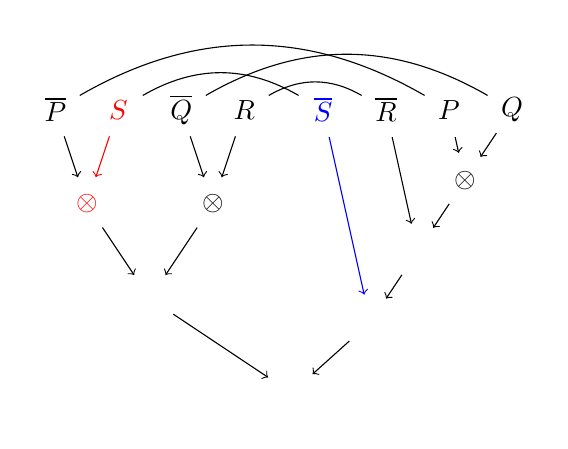
\begin{tikzpicture}
  \tikzstyle{every node}=[circle, minimum size=20pt, inner sep=2pt]
  \draw (0, 0) node (par1) {$\parr$};
  \draw (1, 0.9) node (par3) {\color{blue} $\parr$};
  \draw (-1.8, 1.2) node (par2) {$\parr$};
  \draw (-2.6, 2.4) node (tens1) {\color{red} $\otimes$};
  \draw (-1, 2.4) node (tens2) {$\otimes$};
  \draw (-2.2, 3.6) node (S) {\color{red} $S$};
  \draw (-0.6, 3.6) node (R) {$R$};
  \draw (-3, 3.6) node (nP) {$\overline{P}$};
  \draw (-1.4, 3.6) node (nQ) {$\overline{Q}$};
  \draw (0.4, 3.6) node (nS) {\color{blue} $\overline{S}$};
  \draw (1.6, 1.8) node (par4) {$\parr$};
  \draw (2.2, 2.7) node (tens3) {$\otimes$};
  \draw (2, 3.6) node (P) {$P$};
  \draw (2.8, 3.6) node (Q) {$Q$};
  \draw (1.2, 3.6) node (nR) {$\overline{R}$};
  \draw (par2) -- (par1) [->];
  \draw (par3) -- (par1) [->];
  \draw (tens1) -- (par2) [->];
  \draw (tens2) -- (par2) [->];
  \draw (nP) -- (tens1) [->];
  \draw (S) -- (tens1) [->, color=red];
  \draw (nQ) -- (tens2) [->];
  \draw (R) -- (tens2) [->];
  \draw (nS) -- (par3) [->, color=blue];
  \draw (nR) -- (par4) [->];
  \draw (tens3) -- (par4) [->];
  \draw (P) -- (tens3) [->];
  \draw (Q) -- (tens3) [->];
  \draw (par4) -- (par3) [->];
  \draw (nP) to [bend left] (P);
  \draw (nQ) to [bend left] (Q);
  \draw (S) to [bend left] (nS);
  \draw (R) to [bend left] (nR);
\end{tikzpicture}
}

{\bf Figure 8.} The unification net in Example \ref{exunif} and its frame. The colored part shows how the dependency ${\color{red} \exists x} \rightarrow {\color{blue} \forall z}$ is transformed.
\end{center}

We have the following results: 

Let $u$ and $v$ be atoms or quantifiers in a unification structure $\theta$. Then they are connected by a switching path in the unification structure if, and only if, their corresponding nodes are connected by a switching path in $\theta_m$.

Consider now a switching graph $H$ of a unification structure $\theta$ of $\phi$.

If $H$ contains a cycle, then the corresponding switching graph of $\theta_m$ also contains a cycle. Hence, by applying the propositional results (Theorem 7) from \cite{Retore 2003}, we conclude that there exists a chordless, alternating, and elementary cycle in the bicoloured graph ($W, E_W \uplus L_W$), which corresponds to an induced bimatching in the linked fograph. (Note that the linked fograph (cograph) corresponding to $\theta_m$ is equivalent to the one corresponding to $\theta$.)


\iffalse
Consider a switching graph.
We associate to this switching graph a proof net for {\bf MLL} by replacing quantifiers with fresh atoms and dependencies with new axiom links using the following schema:

\begin{center}	
\mbox{
    \begin{tikzpicture}
    \tikzstyle{every node}=[circle, minimum size=12pt, inner sep=2pt]
    \draw (0, -2) node (existsx) {$\exists x$};
    \draw (0, 0) node (A) {$A$};
    \draw (existsx) -- (A) ;
    \end{tikzpicture}
    
    \vspace{0.5cm}
    \begin{tikzpicture}
    \draw (0, 1) node
    {$\leadsto$};
    \draw (0, 2) node {};
    \draw (0, 0) node {};
    \end{tikzpicture}
    \vspace{0.5cm}
    
    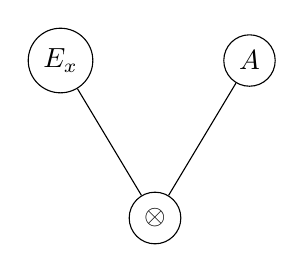
\begin{tikzpicture}
    \tikzstyle{every node}=[draw, circle, minimum size= 12 pt, inner sep=3pt]
    \draw (0, 0) node (existx) {$E_x$};
    \draw (1.2, -2) node (tens) {$\otimes$};
    \draw (2.4, 0) node (A) {$A$};
    \draw (tens) -- (A);
    \draw (tens) -- (existx);
    \end{tikzpicture}
}
\vspace{0.3cm}

\mbox{
    \begin{tikzpicture}
    \tikzstyle{every node}=[circle, minimum size=12pt, inner sep=2pt]
    \draw (0, -2) node (forallx) {$\forall x$};
    \draw (0, 0) node (A) {$A$};
    \draw (forallx) -- (A) ;
    \end{tikzpicture}
    
    \vspace{0.5cm}
    \begin{tikzpicture}
    \draw (0, 1) node
    {$\leadsto$};
    \draw (0, 2) node {};
    \draw (0, 0) node {};
    \end{tikzpicture}
    \vspace{0.5cm}
    
    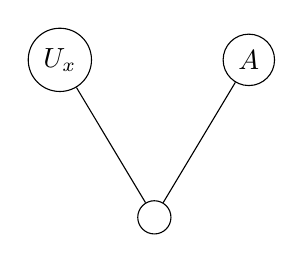
\begin{tikzpicture}
    \tikzstyle{every node}=[draw, circle, minimum size= 12 pt, inner sep=3pt]
     \draw (0, 0) node (Ux) {$U_x$};
    \draw (1.2, -2) node (parr) {$\parr$};
    \draw (2.4, 0) node (A) {$A$};
    \draw (parr) -- (A);
    \draw (parr) -- (Ux);
    \end{tikzpicture}
}

\mbox{
    \begin{tikzpicture}
    \tikzstyle{every node}=[circle, minimum size=12pt, inner sep=2pt]
    \draw (-2, -2) node (existsx) {$\exists x$};
    \draw (-2, 0) node (A) {$A$}; 
    \draw (0, -2) node (forally) {$\forall y$};
    \draw (0, 0) node (B) {$B$};
    \draw (forally) -- (B);
    \draw (existsx) -- (A);
    \draw[->] (existsx) -- (forally);
    \end{tikzpicture}
    
    \vspace{0.5cm}
    \begin{tikzpicture}
    \draw (0, 1) node
    {$\leadsto$};
    \draw (0, 2) node {};
    \draw (0, 0) node {};
    \end{tikzpicture}
    \vspace{0.5cm}
    
    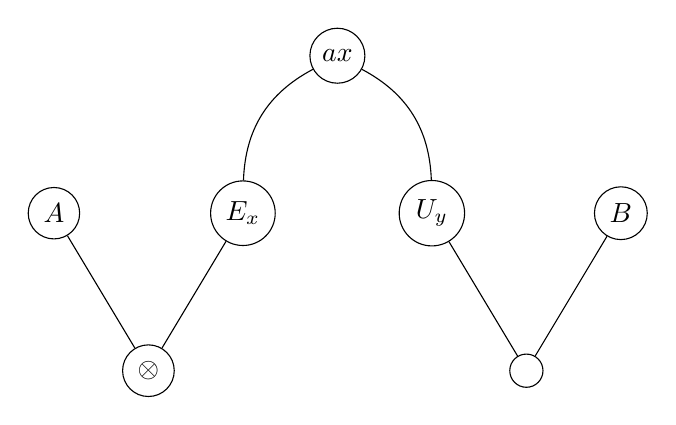
\begin{tikzpicture}
    \tikzstyle{every node}=[draw, circle, minimum size= 12 pt, inner sep=3pt]
    \draw (4.8, 0) node (Uy) {$U_y$};
    \draw (6, -2) node (parr) {$\parr$};
    \draw (7.2, 0) node (B) {$B$};
    \draw (parr) -- (B);
    \draw (parr) -- (Uy);
    \draw (2.4, 0) node (existx) {$E_x$};
    \draw (1.2, -2) node (tens) {$\otimes$};
    \draw (0, 0) node (A) {$A$};
    \draw (tens) -- (A);
    \draw (tens) -- (existx);
    \draw (3.6, 2) node (ax) {$ax$};
    \draw (ax) to [bend right] (existx);
    \draw (ax) to [bend left] (Uy);
   
    
    \end{tikzpicture}
}
\end{center}
\fi



\end{proof}

\iffalse

\begin{proof}
Let $C$ be a cycle contained in a switching graph. We can suppose that $C$ is
minimum, i.e., for all $V' \subsetneq V $, there is no cycle going through exactly $V'$ in a switching graph of the unification structure, where $V$ is the set of vertices of $C$. 

Now write $C$ as the
concatenation of $l_1, p_1, l_2, p_2, ..., l_n, p_n$ where the $l_i$ are
leaps and the $p_i$ are paths consisting of the other edges. We first prove that
for all $i$, $p_i$ is non-empty.

Suppose that $p_k$ is empty. The only possible case is:
\begin{center}
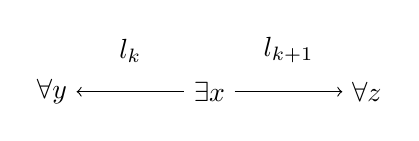
\begin{tikzpicture}
  \node (x0) at (0, 0) {$\forall y$};
  \node (x1) at (2, 0) {$\exists x$};
  \node (x2) at (4, 0) {$\forall z$}; 
  \draw [->] (x1) -- (x0) node [midway, above=7pt] {$l_k$};
  \draw [->] (x1) -- (x2) node [midway, above=7pt] {$l_{k+1}$};
\end{tikzpicture}
\end{center}

This means that every unifier of the unification structure assigns a term
containing $y$ and $z$ to the existential binder $x$, which also implies
the existence of an atom which is a descendant of the $\exists x$. Without loss of
generality, we can assume that the predual of this atom is in the scope
of $\forall y$, then it must contain $y$ and $z$, which is contradictory.

Hence, all the $p_i$ are non-empty.

Let $u_i$ and $v_i$ be the two extremes of the path $p_i$. Since $C$ is
elementary, $u_i$ and $v_i$ are distinct. If one of them, say $u_i$, is a
universal quantifier $\forall x$, then $v_i$ is not in its scope. In fact, since a
dependency edge incident to $\forall x$ is in the switching graph, the
incoming edge from the direct subterm of $\forall x$ to $\forall x$ in the
unification structure is removed in the switching graph.\\
Hence, $u_i$ and $v_i$ are adjacent in the corresponding fograph by proposition
\ref{prop2}.

We now prove that $W = \{u_i | 1 \leq i \leq n \} \cup \{v_i | 1 \leq i \leq n \}$ induces a bimatching in the corresponding linked fograph.

If $u_i$ and $u_j$ (resp. $v_j$ ($i \neq j$) are adjacent in the fograph, then $C$ is not minimum. Hence $u_i$ and $v_i$ are the only neighbours to each other in the fograph.

The reasoning for proving that $p_k$ is non-empty also proves that every existential quantifier has a unique neighbour in the leap graph. The uniqueness of neighbours of universal quantifiers in the leap graph is guaranteed by the definition of switching graph.

\end{proof}
\fi
\end{proposition}

\subsection{From contraction/weakening to skew bifibrations}

We first introduce the atomic contraction rule, the medial rule, and two rules
on quantifiers.

\begin{center}
\mbox{
\begin{prooftree}
  \hypo{\vdash S\{a \vee a\}}
  \infer1[$\acD$]{\vdash S\{a\}}
\end{prooftree}
\hspace{0.3cm}

\begin{prooftree}
  \hypo{\vdash S\{(A \wedge B) \vee (C \wedge D)\}}
  \infer1[$\me$]{\vdash S\{(A \vee C) \wedge (B \vee D)\}}
\end{prooftree}
\hspace{0.3cm}

\begin{prooftree}
  \hypo{\vdash S\{\exists x A \vee \exists x B\}}
  \infer1[$\mee$]{\vdash S\{\exists x (A \vee B)\}}
\end{prooftree}	
\hspace{0.3cm}

\begin{prooftree}
  \hypo{\vdash S\{\forall x A \vee \forall x B\}}
  \infer1[$\meee$]{\vdash S\{\forall x (A \vee B)\}}
\end{prooftree}	
}
\end{center}

Here, we also consider the equivalence generated by the associativity, commutativity of $\vee$ and the equations $\ttt \vee A \equiv \ttt$ and $\fff \vee A \equiv A$.

Now we have the following lemma:

\begin{lemma}
\label{lemma_ctr}
The contraction rule $\cD$ is derivable for $\{\acD, \me, \mee, \meee\}$.
\end{lemma}
\begin{proof}
	We prove that there is always $\vlderivation{\vlde{}{\{\acD, \me, \mee,
	\meee\}}{A}{\vlhy {A \vee A}}}$ by structural induction on $A$.
\begin{itemize}
  \item If $A = \ttt$ or $A = \fff$, we have 
	  \begin{prooftree} 
	    \hypo{\vdash S\{A \vee A\}}
	    \infer1[$\equiv$]{\vdash S\{A\}}
	  \end{prooftree}. (the premiss and the conclusion are equivalent)
  \item If $A = a$, then we have 
	  \begin{prooftree}
	    \hypo{\vdash S\{a \vee a\}}
	    \infer1[$\acD$]{\vdash S\{a\}}.
	  \end{prooftree}
  \item If $A = A_1 \vee A_2$, then by the induction hypothesis, we have 
	  $\vlderivation{\vlde{}{\{\acD, \me, \mee,
	\meee\}}{A_i}{\vlhy {A_i \vee A_i}}}$ for $i = 1, 2$.
	
	Hence, we have
	\begin{prooftree}
	  \hypo{\vdash S\{(A_1 \vee A_2) \vee (A_1 \vee A_2)\}}
	  \infer1[$\equiv$]{\vdash S\{(A_1 \vee A_1) \vee (A_2 \vee A_2)\}}
	  \ellipsis{$\{\acD, \me, \mee, \meee\}$}
		   {\vdash S\{A_1 \vee (A_2 \vee A_2)\}}
	  \ellipsis{$\{\acD, \me, \mee, \meee\}$}
		   {\vdash S\{A_1 \vee A_2\}}
	\end{prooftree}
  \item If $A = A_1 \wedge A_2$, then by the induction hypothesis, we have 
$\vlderivation{\vlde{}{\{\acD, \me, \mee, \meee\}}{A_i}
	      {\vlhy {A_i \vee A_i}}}$ for $i = 1, 2$.

 	Hence, we have
	\begin{prooftree}
	  \hypo{\vdash S\{(A_1 \wedge A_2) \vee (A_1 \wedge A_2)\}}
	  \infer1[$\me$]{\vdash S\{(A_1 \vee A_1) \wedge (A_2 \vee A_2)\}}
	  \ellipsis{$\{\acD, \me, \mee, \meee\}$}
		   {\vdash S\{A_1 \wedge (A_2 \vee A_2)\}}
	  \ellipsis{$\{\acD, \me, \mee, \meee\}$}
		   {\vdash S\{A_1 \wedge A_2\}}
	\end{prooftree}
  \item If $A = \exists x A'$, then by the induction hypothesis, we have $\vlderivation{\vlde{}{\{\acD, \me, \mee,
	\meee\}}{A'}{\vlhy {A' \vee A'}}}$.

	Hence, we have
	\begin{prooftree}
	  \hypo{\vdash S\{\exists x A' \vee \exists x A'\}}
 	  \infer1[$\mee$]{\vdash S\{\exists x (A' \vee A')\}}
	  \ellipsis{$\{\acD, \me, \mee, \meee\}$}
		   {\vdash S\{\exists x A'\}}
	\end{prooftree}
  \item If $A = \forall x A'$, then by the induction hypothesis, we have $\vlderivation{\vlde{}{\{\acD, \me, \mee,
	\meee\}}{A'}{\vlhy {A' \vee A'}}}$.

	Hence, we have
	\begin{prooftree}
	  \hypo{\vdash S\{\forall x A' \vee \forall x A'\}}
 	  \infer1[$\meee$]{\vdash S\{\forall x (A' \vee A')\}}
	  \ellipsis{$\{\acD, \me, \mee, \meee\}$}
		   {\vdash S\{\forall x A'\}}
	\end{prooftree}

\end{itemize}

\end{proof}

\begin{lemma}
The rules $\mee$ and $\meee$ are derivable for $\{\wD, \cD\}$.
\end{lemma}

\begin{proof}
We have:
\begin{center}
\begin{prooftree}
\hypo{\exists x A}
\infer1[$\equiv$]{\exists x (A \vee \fff)}
\infer1[$\wD$]{\exists x (A \vee B)}
\end{prooftree}
\hspace{0.5cm}
and 
\hspace{0.5cm}
\begin{prooftree}
\hypo{\exists x B}
\infer1[$\equiv$]{\exists x (\fff \vee B)}
\infer1[$\wD$]{\exists x (A \vee B)}
\end{prooftree}
\end{center}
Thus, we have:

\begin{center}
\begin{prooftree}
\hypo{\exists x A \vee \exists x B}
\ellipsis{}{\exists x (A \vee B) \vee \exists x (A \vee B)}
\infer1[$\cD$]{\exists x (A \vee B)}
\end{prooftree}
\end{center}
Similar for $\meee$.
\end{proof}

Now we define a propositional encoding for first-order formulas.

\begin{definition}
The propositional encoding $A^P$ of a formula $A$ is defined inductively by:

\begin{centering}
	$a^P = a$ for every atom $a$

	$(A \vee B)^P = A^P \vee B^P$ \hspace{2cm} $(A \wedge B)^P = A^P \wedge B^P$

	$(\forall x A)^P = U_x \vee A^P$ \hspace{2cm} $(\exists x A)^P = E_x \wedge A^P$

\end{centering}
where $U_x$ and $E_x$ are fresh nullary atoms.

\end{definition}

Similarly, we can define the propositional encoding $S^P$ of a context $S$ inductively by setting $\Box^P = \Box$. Note that $S^P$ is also an encoding.

We have the following facts:

\begin{proposition}
For any context $S$ and any formula $A$:
\begin{itemize}
  \item $A^P$ is a formula containing no quantifier for any formula $A$.
  \item $G(A^P) = G(A)$ by confounding the atoms $U_x$, $E_x$ with the variable
	  $x$. Thus, a map $f : G(A^P) \rightarrow G(B^P)$ can be seen as a map
		$f : G(A) \rightarrow G(B)$.
  \item $(S\{A\})^P = S^P\{A^P\}$.
\end{itemize}

\end{proposition}

\begin{proposition}
\label{prop311}
Let $A$ and $B$ be two formulas such that
$\od{\odd{\odh {A}}{}{B}{\{\wD, \cD\}}}$. Then 
$\od{\odd{\odh {A^P}}{}{B^P}{\{\wD, \cD\}}}$.
\end{proposition}

\iffalse
\begin{proof}

We say that a rule \begin{prooftree} \hypo{C} \infer1[]{D} \end{prooftree}
is $P$-derivable for $\{\wD, \cD\}$ if
        $\od{\odd{\odh {C^P}}{}{D^P}{\{\wD, \cD\}}}$.

We now prove that $\wD$ and $\cD$ are
	$P$-derivable for $\{\wD, \cD\}$. 

\begin{itemize}
\item $\wD$ is $P$-derivable: we have
  \begin{prooftree}
    \hypo{S^P\{\fff\}}
    \infer1[$\wD$]{S^P\{C^P\}}
  \end{prooftree}

\item $\cD$ is $P$-derivable: we have
  \begin{prooftree}
    \hypo{S^P\{C^P \vee C^P\}}
    \infer1[$\cD$]{S^P\{C^P\}}
  \end{prooftree}

\end{itemize}

Hence, $\od{\odd{\odh {A^P}}{}{B^P}{\{\wD, \cD\}}}$.

\end{proof}
\fi

\begin{lemma}
\label{mlem}
	Given two formulas $A$ and $B$ and a derivation $\od{\odd{\odh {A}}
	{\Delta}{B}{\{\wD, \cD\}}}$, then there exists a skew bifibration $G(A)
	\rightarrow G(B)$.
\end{lemma}

\begin{proof}
By Lemma \ref{lemma_ctr}, there exists a derivation $\od{\odd{\odh {A}}
	{\Delta}{B}{\{\wD, \acD, \me, \mee, \meee \}}}$.
	
For each rule from $\{\wD, \acD, \me, \mee, \meee \}$, we define a map and show that it is a skew fibration.

\begin{itemize}
  \item \begin{prooftree}
  \hypo{\vdash S\{\fff \}}
  \infer1[$\wD$]{\vdash S\{A\}}
\end{prooftree}:

  the map $wk$ maps $\fff$ to anything and is identity elsewhere.   
  
  \item
    \begin{prooftree}
      \hypo{\vdash S\{a \vee a\}}
       \infer1[$\acD$]{\vdash S\{a\}} 
    \end{prooftree}: 
    
    the map $ac$ maps the two $a$-labelled literals in the premise to the $a$-labelled literal in the conclusion.

  \item 
    \begin{prooftree}
      \hypo{\vdash S\{(A \wedge B) \vee (C \wedge D)\}}
      \infer1[$\me$]{\vdash S\{(A \vee C) \wedge (B \vee D)\}}
    \end{prooftree}:
    
    the map $m$ is the canonical identity that maps $A$ to $A$, $\cdots$, $D$ to $D$.
  \item 
    \begin{prooftree}
      \hypo{\vdash S\{\exists x A \vee \exists x B\}}
      \infer1[$\mee$]{\vdash S\{\exists x (A \vee B)\}}
    \end{prooftree}: 
   
    the map $m_1$ maps the two $x$-labelled binders in the premise to the $x$-labelled binder in the conclusion,  $A$ to $A$ and $B$ to $B$.
  \item
    \begin{prooftree}
      \hypo{\vdash S\{\forall x A \vee \forall x B\}}
      \infer1[$\meee$]{\vdash S\{\forall x (A \vee B)\}}
    \end{prooftree}:
    
    the map $m_2$ maps the two $x$-labelled binders in the premise to the $x$-labelled binder in the conclusion,  $A$ to $A$ and $B$ to $B$. 

\end{itemize}

By considering propositional encodings, the maps defined are label-preserving skew fibrations on the underlying fographs according to \cite{Strassburger 2007}.

Now we prove that each map $g \in \{wk, ac, m, m_1, m_2 \}$ is a skew bifibration. To do that, it suffices to prove that $g$ is a fibration between the corresponding binding graphs since it is already a skew fibration on the corresponding fographs and it is label-preserving and existential-preserving.
\begin{center}
	for each $x$-binder $b$ in $G(B^P)$, for each vertex $v \in V(G(A^P))$
such that $g(v)$ is bound by $b$, there exists a unique binder $b'$ such
that $b'$ binds $v$.
\end{center}

\begin{itemize}
  \item $wk$ and $m$ are clearly fibrations: the binding relations of the premise and the conclusion are exactly the same.
  \item $ac$ is a fibration: suppose that $a$ that in the conclusion $a$ is bound by some quantifier $b$ in $S$, then for each of its preimages by $ac$, there exists exactly one binder (in fact, $b$) in $S$ that binds it.
  \item $m_1$ and $m_2$ are fibrations: in the conclusion, for every atom $a$ in $A \vee B$ bound by the $x$-labelled quantifier, $a$ has exactly one preimage and it is bound by the $x$-llabelled quantifier in the premise.
\end{itemize}

  Therefore, all of these maps are skew bifibrations and since skew bifibrations on fographs compose (Lemma 10.32, \cite{Hughes 2019}), there exists a skew bifibration from $G(A)$ to $G(B)$.

\iffalse

By Proposition \ref{prop311}, $\od{\odd{\odh {A^P}}{}{B^P}{\{\wD, \cD\}}}$.
Since both $A^P$ and $B^P$ are propositional (without quantifier), we
can place ourselves in a propositional setting. We have thus a skew
fibration $f$ from $G(A^P) = G(A)$ to $G(B^P) = G(B)$ by Theorem 7.8
of \cite{Strassburger 2007}. To check that it is a skew bifibration, it suffices to check that:
\begin{center}
	for each $x$-binder $b$ in $G(B^P)$, for each vertex $v \in V(G(A^P))$
such that $f(v)$ is bound by $b$, there exists a unique binder $b'$ such
that $b'$ binds $v$.
\end{center}
	
According to \cite{Strassburger 2007}, a such map $f$ can be seen as a
composition of:
\begin{itemize}
  \item an identity map on labels $i: G(A^P) \rightarrow G(C)$ which is a skew fibration,
  \item a label-preserving atomic contraction map $c: G(C) \rightarrow G(D)$, i.e., a
	surjective skew fibration such that for all $u, v \in V_{G(C)}$,
	we have $u \frown_{C} v$ iff $c(u) \frown_{D} c(v)$, and
  \item a label-preserving weakening map $w: G(D) \rightarrow G(B^P)$, i.e., an
	injective skew fibration such that for all $u, v \in V_{G(D)}$, we have 
	$u \frown_{D} v$ iff $w(u) \frown_{B^P} w(v)$.

\end{itemize}
Here, $u \frown_{C} v$ means that the first common ancestor of $u$ and $v$ in
the "propositional" formula $C$ is a $\wedge$, i.e., $u$ and $v$ are adjacent in
$G(C)$. 

	Let $b$ be an $x$-binder in $G(B)$ and let $v \in V_{G(A^P)}$. Suppose that $f(v)$ is bound by $b$. 

We distinguish two cases:
\begin{itemize}
	\item $b$ is existential: $b$ and $f(v)$ are adjacent in $V_{G(B)}$ since
	$f(v)$ is in the scope of $b$ and its atom contains $x$. Hence, the
	$E_x$-labelled vertex $u$ corresponding to $b$ is such that
	$u \frown_{B^P} f(v) = w(c(v))$. \\
	Now we prove that $u$ is in the image of $w$. Since $w$ is a skew
	fibration, there exists $\tilde{u} \in V_{G(D)}$ such that
		$\tilde{u} \frown_{D} c(v)$ and $w(\tilde{u}) \nfrown_{B^P} u$.
	Suppose that $w(\tilde{u}) \neq u$.
	We distinguish two cases:
	\begin{itemize}
	  \item $w(\tilde{u})$ corresponds to a descendant of $b$ in $B$: we have $w(\tilde{u}) \frown_{B^P} u$ by definition of $B^P$, which is contradictory.
	  \item $w(\tilde{u})$ does not correspond to a descendant of $b$ in $B$: this implies that in $B^P$, $b$ is a descendant of the first common ancestor of $w(\tilde{u})$ and $f(v)$ . We have also $w(\tilde{u}) \frown {B^P} f(v)$. Hence, the first common ancestor of $b$ and $w(\tilde{u})$ is equal to the latter. We have thus $w(\tilde{u}) \frown_{B^P}$, which is again contradictory.
  \end{itemize}
  Hence, $w(\tilde{u}) = u$.
  And since $w$ is injective, such $\tilde{u}$ is unique.
  We have thus a unique u such that $w(\tilde{u}) \frown_{B^P} f(v) = w(c(v))$, which is equivalent to $\tilde{u} \frown_{D} c(v)$. Since $c$ is a skew fibration, there exists $\tilde{\tilde{u}} \in V_(G(C))$ such that $\tilde{\tilde{u}} \frown{C} v$ and 
  $c(\tilde{\tilde{u}}) \nfrown_{D} \tilde{u}$.
  The same reasoning as the previous one proves that $c(\tilde{\tilde{u}}) = \tilde{u}$.  
  \item 
\end{itemize}

\fi

\end{proof}

\begin{theorem_}
If a formula $\phi$ is provable in {\bf LK}, then it has a combinatorial proof.
\end{theorem_}

\begin{proof}
By Theorem \ref{thm1}, there exists a formula $\phi'$ such that there is a proof $\Pi$ of $\phi'$ in {\bf MLL1} and a derivation $D$ from $\phi'$ to $\phi$ consisting of the $\wD$ and $\cD$ rules only. The proof $\Pi$ corresponds to a unique unification net which is equivalent to the fonet corresponding to $\Pi$, i.e., the fograph $G(\phi')$ together with the links of $\Pi$. By Lemma \ref{mlem}, there exists a skew bifibration $G(\phi') \rightarrow G(\phi)$. We have thus a combinatorial proof of $\phi$.

\end{proof}

\subsection{From skew bifibrations to contraction/weakening}

\begin{theorem_}
Let $A$ and $B$ be two formulas and $f: G(A) \rightarrow G(B)$ a skew bifibration. Then there exists a derivation $\od{\odd{\odh {A}}{\Delta}{B}{\{\wD, \cD\}}}$.
\end{theorem_}

$f$ can be seen as a skew fibration from $G(A^P)$ to $G(B^P)$, which gives the existence of the propositions $A'$ and $B'$, and of the following derivation:
  \[\od{\odd{\odd{\odd{\odh{A^P} }
  {\Delta }{A'}{\me} }
  {\Delta' }{B'}{\acD} }
  {\Delta''}{B^P}{\wD}} \]

\begin{lemma} there exists $B''$ such that $B''^P$ = $B'$.

\begin{proof}
Consider the dervation $\Delta''$. If some $U_x$ (or $E_x$) is introduced
via weakening, then all the atoms it binds in $B^P$ should also be introduced 
via weakening. In fact, an atom of $B^P$ is introduced via weakening is 
equivalent to the fact that its corresponding vertex is not in the image of $f$. 
Since there is an edge from $U_x$ (resp. $E_x$) to all the literals it binds in the 
binding graph $\overrightarrow{G(B)}$, if one of the atoms is in the image, 
$U_x$ (resp. $E_x$) should also be in the image since $f$ is a fibration on binding graphs.

This means that a such $B''$ can be obtained from $B$ by erasing all the $U_x$ and $E_x$ introduced via weakening and all the atoms they bind.
\end{proof}
\end{lemma}

We introduce new (atomic) symbols $E_x^*$ and $U_x^*$ which are used to
represent disjunctions of $E_x$ and $U_x$ respectiveley.

We define a translation $(\cdot)^*$ inductively by:
\begin{itemize}
  \item $(E_x \vee \cdots \vee E_x)* = E_x^*$
  \item $(U_x \vee \cdots \vee U_x)* = U_x^*$
  \item structural recursion in all the other cases.
\end{itemize}

Then the derivation:
 \[\od{\odd{\odd{\odh{A^P} }
  {\Delta }{A'}{\me} }
  {\Delta' }{B'}{\acD}} \]
can be translated to the derivation:
\[\od{\odd{\odh{(A^P)^*} }
{\Delta^* }{(B')^*}{}} \]

where $\Delta^*$ is the derivation obtained by replacing all the formulas $F$
with $F^*$.

Note that we should also introduce new rules in the derivation $\Delta^*$.
Otherwise, the rule applications cannot work in general.

To do that, we define the following rule transformation:

\begin{center}
\mbox{
\begin{prooftree}
  \hypo{Q_x^*}
  \infer1[$\acD$]{Q_x^*}
\end{prooftree}

$\leadsto$

\begin{prooftree}
  \hypo{Q_x^*}
  \infer1[$=$]{Q_x^*}
\end{prooftree}

}
\vspace{0.4cm}

\mbox{
\begin{prooftree}
  \hypo{(Q_x^* \wedge C) \vee (Q_x^* \wedge D)}
  \infer1[$\me$]{Q_x^* \wedge (C \vee D)}
\end{prooftree}

$\leadsto$

\begin{prooftree}
  \hypo{(Q_x^* \wedge C) \vee (Q_x^* \wedge D)}
  \infer1[$\me'$]{Q_x^* \wedge (C \vee D)}
\end{prooftree}

}
	
\end{center}
where $Q_x^*$ stands for $E_x^*$ or $U_x^*$.

$\Delta^*$ can now be transformed into a valid derivation $\Delta_1$ by using the two
transformation rules above and by applying them in a bottom-up style:
\[\od{\odd{\odh{(A^P)^*} }
{\Delta_1 }{(B')^*}{\acD, \me, \me'}} \]

\begin{lemma}
Every line of $\Delta_1$ is a propositional encoding (by
confounding $Q_x^*$ with $Q_x$).

\begin{proof}
We proceed by bottom-up induction in the derivation.
Clearly, $B'*$ is a propositional encoding as there is no disjunction of $Q_x$
in it.

First consider the $\acD$ rule:
\begin{prooftree}
  \hypo{C \vee C}
  \infer1[$\acD$]{C}
\end{prooftree}

It is clear that if $C$ is a propositional encoding, then so is $C \vee C$.

Now consider the $\me$ rule:
\begin{prooftree}
  \hypo{(C \wedge D) \vee (E \wedge F)}
  \infer1[$\me$]{(C \vee E) \wedge (D \vee F)}
\end{prooftree}

Suppose that $(C \vee E) \wedge (D \vee F) = G^P$ for some $G$.
Since $C \vee E$ cannot be $Q_x$ (otherwise, the rule applied would be
$\me'$), $G$ can be written as $G_1 \wedge G_2$ with $C \vee E = G_1^P$ and $D
\vee F = G_2^P$.

We have thus $G_i = \forall x_i H_i$ or $J_i \vee K_i (i = 1, 2)$.

If $G_i = \forall x H_i$ for some $i$, then there will be a conjunction of $U_x^*$
and some formula which can never be eliminated by the rules $\me$, $\me'$ and
$\acD$. However, there exists no such conjunction in ${A^P}^*$, which leads to a
contradiction.

Hence, $G_i$ can be written as $J_i \vee K_i$ for $i = 1, 2$. We now have $(C
\wedge D) \vee (E \wedge F) = ((J_1 \wedge J_2) \vee (K_1 \wedge K_2))^P$.

Finally, consider the $\me'$ rule:

\begin{prooftree}
  \hypo{(Q_x^* \wedge C) \vee (Q_x^* \wedge D)}
  \infer1[$\me'$]{Q_x^* \wedge (C \vee D)}
\end{prooftree}

Suppose that $Q_X^* \wedge (C \vee D)$ = $F^P$ for some $P$. It is clear
that $Q_x^* = E_x^*$ and $F = \exists x G$ with $G^P = C \vee D$ for some $G$.
We distinguish two cases:
\begin{itemize}
  \item $G = \forall y H$: in this case, $(Q_x^* \wedge C) \vee (Q_x^* \wedge
D)$ has a subformula $(E_x^* \wedge U_y^*)$, which cannot be eliminated by the
rules $\me$, $\me'$, $\acD$. It is clear that ${A^P}^*$ does not
have a subformula of this form, which leads to a contradiction.
  \item $G = G_1 \vee G_2$: in this case, $(Q_x^* \wedge C) \vee (Q_x^* \wedge
	  D) = ((\exists x G_1) \vee (\exists x G_2))^P$.
\end{itemize}

\end{proof}	
\end{lemma}

\end{document}
